\section{Fachklassendiagramm}

\noindent Das folgende Fachklassendiagramm \autoref{fig:Fachklassendiagramm} zeigt die benötigten Klassen mit ihren
Kardinalitäten, Attributen und Operationen für die Umsetzung des \ac{aMRS}. Bei der Modellierung wurden Design Patterns
berücksichtigt, um eine Entkopplung der Komponenten zu verwirklichen. Durch die Entkopplung soll eine bessere
Wartbarkeit, Erweiterbarkeit und die Qualität der Software sichergestellt werden. \newline

\noindent Wie in \autoref{fig:Fachklassendiagramm} zu erkennen ist das System in zwei unabhängige Teilsysteme
untergliedert, welche nur über die Datenspeicherung verbunden sind. Diese nutzt das Repository Pattern, um eine
Entkopplung der Datenzugriffsschicht vom restlichen System zu ermöglichen. Über das Adapter Pattern ist eine
Schnittstelle zwischen Informationsportal und \ac{aMRS} geplant. Zum andern bietet \ac{aMRS} mit ihrer eigenen GUI die
Möglichkeit den im \#TODO autoref ... beschriebenen Bewertungsprozess durchzuführen. Dieser Prozess nutzt einen Adapter
zu einem externen OCR-System und diverse Validatoren, welche mithilfe des Iterator Pattern leicht an zukünftige
Kundenwünsche angepasst werden können.

\newpage

\begin{figure}[H]
    \centering
    \caption{Fachklassendiagramm} \label{fig:Fachklassendiagramm}
    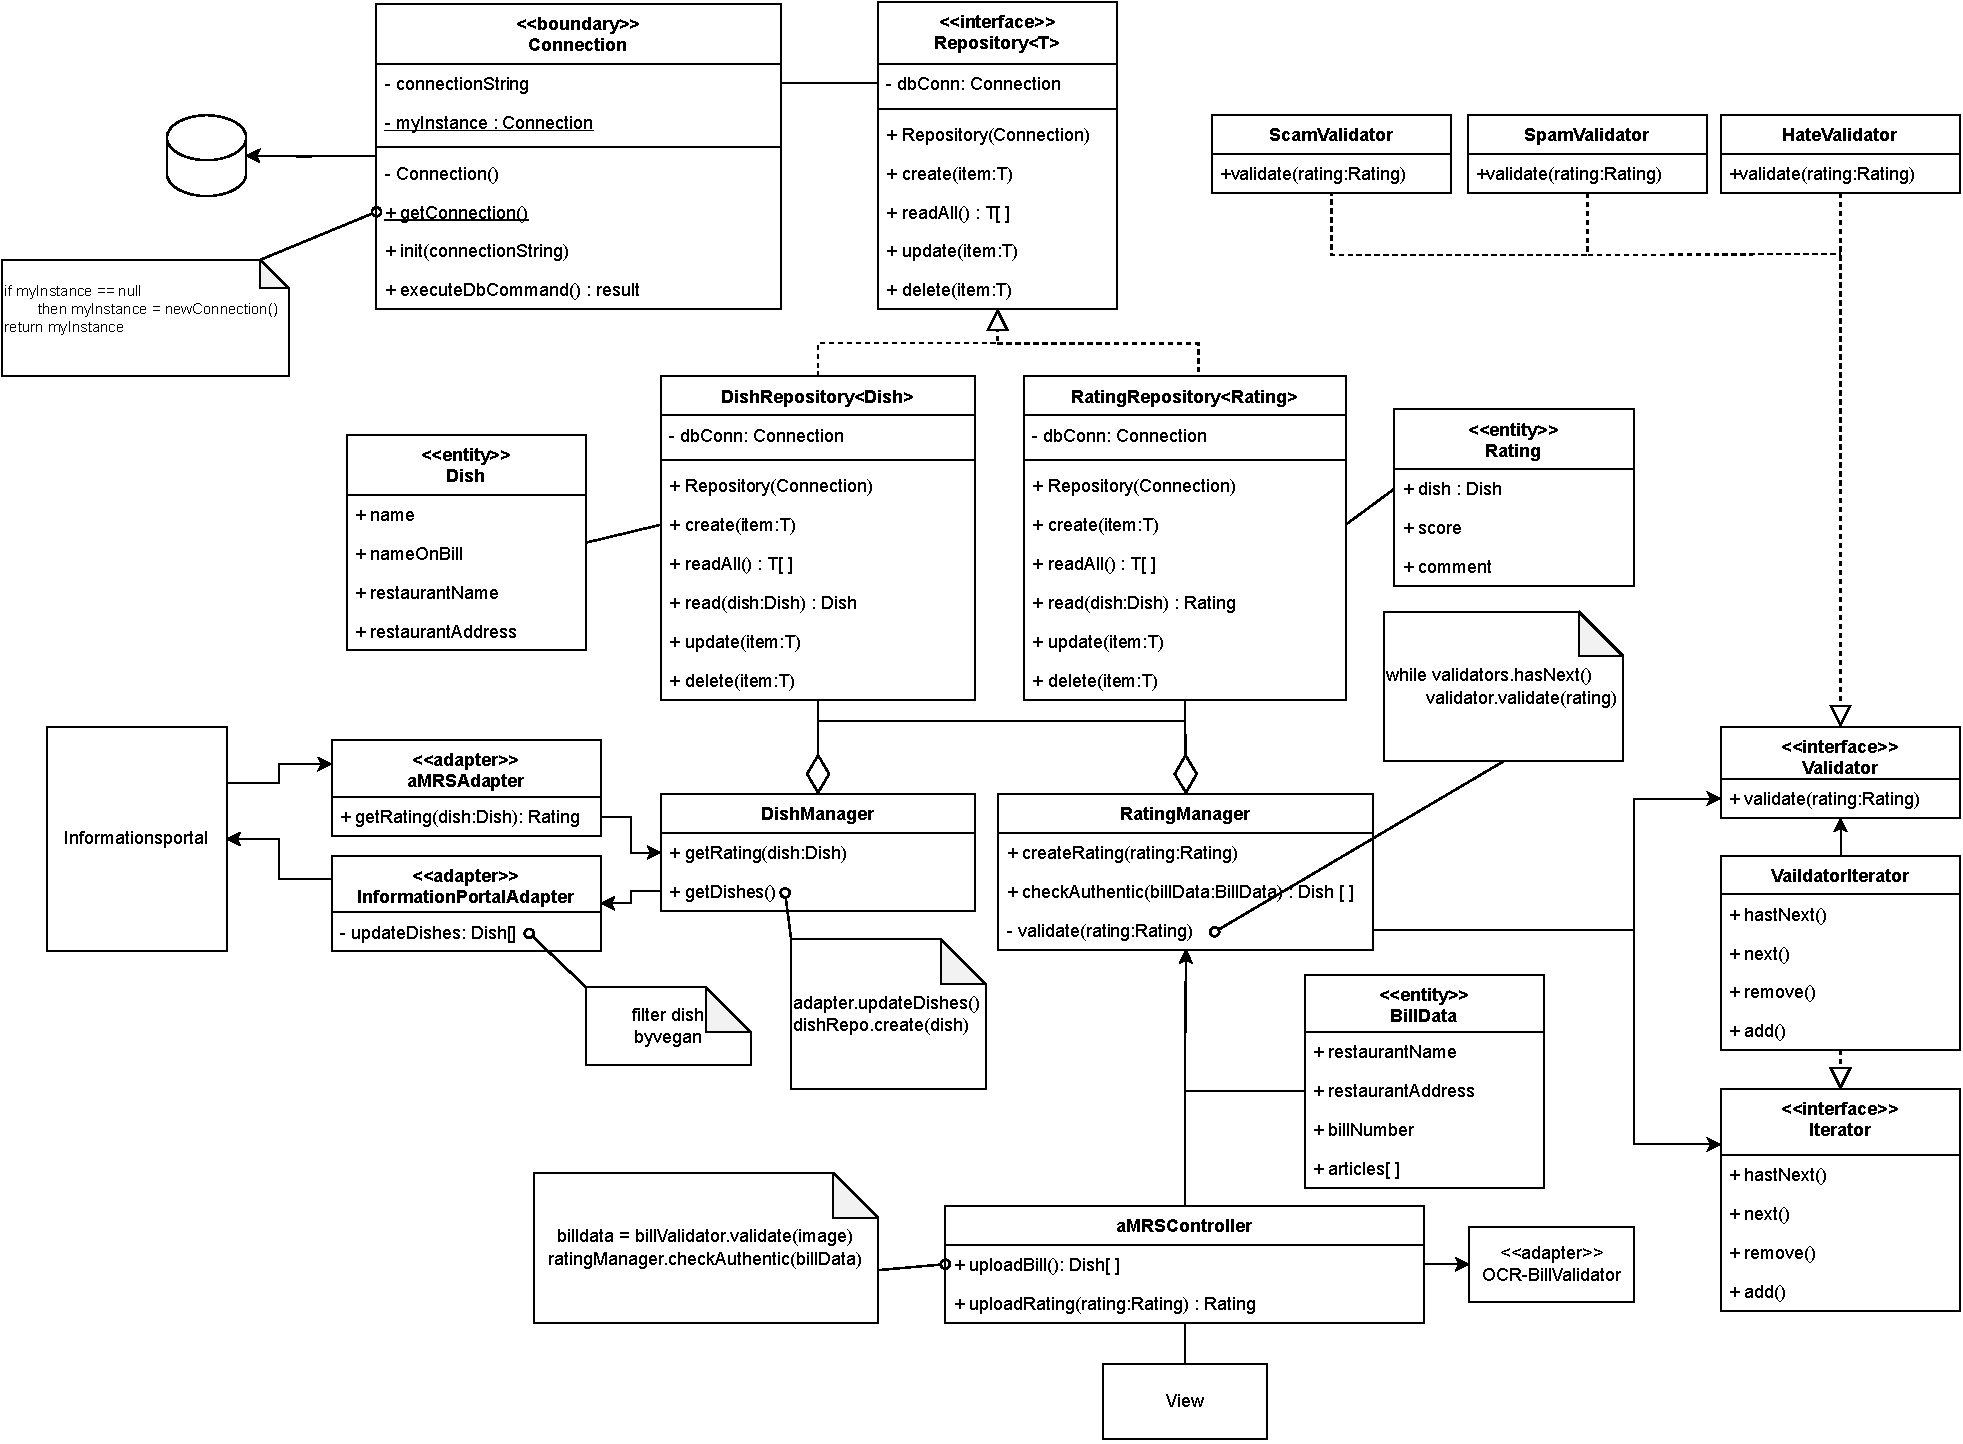
\includegraphics[width=1.3\textwidth,angle=90,keepaspectratio]{images/Fachklassenmodell}
\end{figure}

\section*{Beschreibung der Fachklassen}

\subsection*{Entity}
\textbf{Dish} \\
Die Klasse Dish enthält Informationen über Restaurantname, Restaurantadresse, Rechnungsbezeichner und Gerichtname des
Tagesgerichts.
\newline

\noindent \textbf{BillData} \\
Die Klasse BillData enthält Informationen über Restaurantname, Restaurantadresse, Rechnungsnummer und eine Liste aller
Rechnungsbezeichner der Restaurantrechnung.
\newline

\noindent \textbf{Rating} \\
Die Klasse Rating enthält Informationen über das zu bewertende Dish, eine Wertung und ein Kommentar.

\subsection*{Adapter}
\noindent \textbf{aMRSAdapter}\\
Die Klasse aMRSAdapter gitb dem Informationsportal die Möglichkeit Bewertungen vom \ac{aMRS} abzurufen.
\newline

\noindent \textbf{InformationsPortalAdapter}\\
Die Klasse InformationsPortalAdapter gitb dem \ac{aMRS} die Möglichkeit Tagesgerichte vom Informationsportal abzurufen.
Dabei werden die Tagesgerichte nach Klassifikation gefiltert.
\newline

\noindent \textbf{OCR-BillValidator}\\
Die Klasse OCR-BillValidator stellt die Kommunikation von \ac{aMRS} zum externen OCR-System her.


\subsection*{Boundary}
\noindent \textbf{Connection}\\
Die Klasse Connection empfängt Befehle zur Datenspeicherung beziehungsweise zum Datenzugriff.

\subsection*{Klasse}
\noindent \textbf{DishRepository<Dish>}\\
Die Klasse DishRepository ist für die Speicherung und den Zugriff auf die Daten der Klasse Dish zuständig.
\newline

\noindent \textbf{RatingRepository<Rating>}\\
Die Klasse RatingRepository ist für die Speicherung und den Zugriff auf die Daten der Klasse Rating zuständig.
\newline

\noindent \textbf{DishManager}\\
Die Klasse DishManager enthält die Logik für das Aktualisieren und Speichern neuer Dish-Objekte, sowie zum Abrufen von
vorhandenen Bewertungen.
\newline

\noindent \textbf{RatingManager}\\
Die Klasse RatingManager enthält die Logik für das Speichern und Validieren neuer Rating-Objekte. Zusätzlich wird das
Objekt BillData auf Authentizität überprüft.
\newline

\noindent \textbf{ScamValidator}\\
Die Klasse ScamValidator ist für die Überprüfung auf Scam in Bewertungen zuständig.
\newline

\noindent \textbf{SpamValidator}\\
Die Klasse SpamValidator ist für die Überprüfung auf Spam in Bewertungen zuständig.
\newline

\noindent \textbf{HateValidator}\\
Die Klasse HateValidator ist für die Überprüfung auf Hass in Bewertungen zuständig.
\newline

\noindent \textbf{ValidatorIterator}\\
Die Klasse ValidatorIterator ist für die Iteration über die Validatoren zuständig.
\newline

\noindent \textbf{aMRSController}\\
Die Klasse aMRSController ist für die Kommunikation zwischen View und RatingManager zuständig.
\newline

\noindent \textbf{View}\\
Die Klasse View stellt die GUI dar.